
\subsection{Real Estate Price Model}
\label{sec:real-estate-price-model} \index{Real Estate Price Model}
\modelsindex
%
The \class{RealEstatePriceModel} \modelsindex predicts per-unit prices of buildings, 
for each member of the given
location set. The prediction is done via a regression procedure and thus,
the model \modelsindex is a child of the \class{RegressionModel} \modelsindex described in
Section~\ref{sec:regression-model}.

\subsubsection{Initialization}
%
The class is initialized by passing the following arguments:
\begin{description}
\item[regression_procedure] - a fully qualified name of the module/class in
  which the regression is implemented (see
  Section~\ref{sec:regression}). Default value is
  ``opus_core.linear_regression''.
\item[filter] - name of a variable/attribute used to filter out elements for
  the regression (applied to both, the \method{run()} and \method{estimate()}
  method). Default value is None.
\item[submodel_string] - If model \modelsindex contains submodels, this character string
  specifies what attribute of the observation set determines those
  submodels. Default value is ``building_type_id''.
\item[run_config] - A collection of additional arguments that control a
  simulation run. It should be of class \class{Resources}.
\item[estimate_config] - A collection of additional arguments that control an
  estimation run. It should be of class \class{Resources}.
\end{description}
The constructor sets \verb|filter| as a class attribute \attributesindex and calls the parent
constructor (see Initialization in Section~\ref{sec:regression-model}).

\subsubsection{The Run Method}
%
{\it Input}:\\[1mm]
The \method{run()} method takes exactly the same arguments as its parent
class:\\
{\bf specification}, {\bf coefficients}, {\bf dataset}, \datasetindex {\bf index}, {\bf
  chunk_specification}, {\bf data_objects}, and {\bf run_config}.



{\it Algorithm}:\\[1mm]
If \verb|filter| is given in the initialization, \verb|index| is
updated to only those elements for which the value of
attribute/variable \attributesindex\variablesindex \verb|filter| is
larger than zero. It then invokes the \method{run()} method of
\class{RegressionModel} \modelsindex passing all arguments where
\verb|index| is possibly modified. The returned value of this call
is considered to be the prediction of the natural logarithm of the value 
per unit for each element of \verb|dataset| included in
\verb|index|. The 'unit' used for the predictions is per 'square foot' 
for non-residential buildings, and per residential unit for residential buildings. 
Each of those values is then exponentiated . 
Attribute \attributesindex ``unit_price'' 
 (which is expected to be a known
attribute \attributesindex of the \verb|dataset|) is modified by
replacing current values with the computed values.

If any of the computed values exceeds the maximal value of float32, a warning
is issued and the value is clipped to the maximal possible value.

{\it Output}:\\[1mm]
The method returns an index of values within \verb|dataset| \datasetindex for which the 
unit_price was modified.

\subsubsection{The Estimate Method}
{\it Input}:\\[1mm]
The \method{estimate()} method takes exactly the same arguments as its parent
class: \\
{\bf specification}, {\bf dataset}, \datasetindex {\bf outcome_attribute}, {\bf index}, {\bf
  procedure}, {\bf data_objects}, and {\bf estimate_config}.

{\it Algorithm}:\\[1mm]
The method applies the \verb|filter| (if given) in the same way as the
\method{run()} method. It then calls the parent method \method{estimate()}
passing all arguments and the possible modified \verb|index|.

{\it Output}:\\[1mm]
The method returns results of \method{estimate()} method of
\class{RegressionModel} \modelsindex (see Section~\ref{sec:regression-model}).

\subsubsection{Model Configuration}
\modelsindex
%
{\em Configuration for Production Run}:\\[1mm]
For a production run of UrbanSim the model \modelsindex is
initialized with default values of the model \modelsindex
constructor. The \method{run()} method is called by passing the
following arguments:
\begin{description}
\item[specification] - An
\class{EquationSpecification} object created with data from table
``real_estate_price_model_specification''.  \modelsindex
\item[coefficients] \coefficientsindex - A \class{Coefficients} \coefficientsindex object created
with data from table ``real_estate_price_model_coefficients''. \coefficientsindex\modelsindex
\item[dataset] \datasetindex - An instance of class \class{BuildingDataset} created with data
  from table ``buildings'' (see Section~\ref{sec:parcel-tables} for the
  table structure).
\item[index] - None. Thus, the model \modelsindex runs on all members of \verb|dataset| \datasetindex which are possibly 
filtered using a filter passed to the constructor (by default ``None'', see
the Initialization paragraph).
\end{description}

\subsection{Location Choice Model}
\label{sec:location-choice-model}
\index{Location Choice Model}
A location choice model \modelsindex is a choice model \modelsindex where the set of alternatives is a
set of locations.

The class \class{LocationChoiceModel} \modelsindex is a child of \class{ChoiceModel} \modelsindex
described in Section~\ref{sec:choice-model}. In addition, it allows sampling
of alternatives and filtering alternatives according to a specified filter.

\subsubsection{Initialization}
%
The class is initialized by passing the following arguments:
\begin{description}
\item[location_set] - A dataset \datasetindex of locations to be chosen from.
\item[sampler] - A fully qualified name of the module for sampling
  alternatives. Default value is ``opus_core.samplers.weighted_sampler''. If
  this argument is set to None, no sampling is performed.
\item[utilities] - A fully qualified name of the module for computing utilities
  (see Section~\ref{sec:utilities}). Default value is
  ``opus_core.linear_utilities''.
\item[probabilities] - A fully qualified name of the module for computing
  probabilities (see Section~\ref{sec:probabilities}). Default value is
  ``opus_core.mnl_probabilities''.
\item[choices] - A fully qualified name of the module for determining
  final choices (see Section~\ref{sec:choices}). Default value is
  ``opus_core.random_choices''.
\item[interaction_pkg] - This argument is only relevant if there is an
  explicit implementation of an interaction dataset that corresponds to
  interaction between agents and choices (such as those from
  Table~\ref{tab:urbansim-interaction-datasets}). It then determines the
  package in which the module lives. Default value is
  ``urbansim.datasets''. \datasetindex
\item[filter] - It is either a string specifying an attribute \attributesindex name of the
  filter, or a 1D/2D array giving the filter directly, or a dictionary
  specifying filter for each submodel. If it is None (default), no filter is
  applied.
\item[submodel_string] - If model \modelsindex contains submodels, this character string
  specifies what agent's attribute determines those submodels. If it is None
  (default), no division into submodels is applied.
\item[run_config] - A collection of additional arguments that control a
  simulation run. It should be of class \class{Resources}.
\item[estimate_config] - A collection of additional arguments that control an
  estimation run. It should be of class \class{Resources}.
\end{description}
The method calls the constructor of its parent class. Then, it creates a
\class{Sampler} object from the argument \verb|sampler| using
\class{SamplerFactory}. It sets value of the argument \verb|filter| as a class
property \verb|filter|

%
\subsubsection{The Run Method}
%
The \method{run()} method runs the simulation of location choice model \modelsindex on basis
of a given specification and coefficients. \coefficientsindex

{\it Input}:\\[1mm]
It takes the same arguments as the \method{run()} method of its parent (see
Section~\ref{sec:choice-model} for more details): \\
{\bf specification}, {\bf coefficients}, \coefficientsindex {\bf agent_set}, {\bf agents_index},
{\bf chunk_specification}, {\bf data_objects}, and {\bf run_config}.

{\it Algorithm}:\\[1mm]
The model \modelsindex is processed in chunks. The \method{run_chunk()} method moves
the agents out of their locations, i.e. the values of an
\verb|agent_set| attribute of the same name as the unique identifier of
\verb|location_set| is set to $-1$ for each agents of the currently processed
chunk. If \verb|agent_set| does not have this attribute, \attributesindex it is appended to it.

If an entry ``compute_capacity_flag'' is given in \verb|run_config| and its
value is True, an entry ``capacity_string'' is expected in \verb|run_config|
which gives the name of attribute/variable \attributesindex\variablesindex of \verb|location_set| that
determines capacity for each location. In such a case, after removing agents
from their locations, the capacity is computed using method
\method{determine_units_capacity()}. Note that by removing agents of only the
current chunk from their locations, the capacity is influenced by only those
agents. Each chunk then see the state of the world updated by all previously
running chunks.

The capacity values are used as weights of locations in the case of sampling.
They are multiplied by the filter given in the initialization.  The
model \modelsindex then invokes sampling of alternatives by calling the
\method{run()} method of the sampler class, passing the possibly filtered
weights. The parent class then takes care of creating the interaction set, for
agents of the corresponding chunk and possibly sampled alternatives and of
running the \verb|upc_sequence|. If \verb|run_config| includes an entry
``correct_sampling_bias'' that is set to True, the method performs a bias
correction for non-uniform sampling in the multinomial logit computation.

The location IDs that agents chose in the choice process are stored
in the \verb|agent_set| attribute specifying the location.

{\it Output}:\\[1mm]
The method returns an array of size \verb|agents_index|,
representing the location IDs that agents (elements of
\verb|agent_set| determined by \verb|agents_index|) made. Agents
whose choice is less equal zero were not included in the choice
process, for example because they do not belong to any submodels
given in the specification.


\subsubsection{The Estimate Method}
%
{\it Input}:~\\[1mm]
The \method{estimate()} method takes the same arguments as its parent class:\\
{\bf specification}, {\bf agent_set}, {\bf agents_index}, {\bf procedure},
{\bf data_objects}, and {\bf estimate_config}.

{\it Algorithm}:\\[1mm]
As in the \method{run()} method, if ``compute_capacity_flag'' is given in
\verb|estimate_config| and its value is True, an entry ``capacity_string'' is
expected in \verb|estimate_config| which gives the name of attribute/variable \attributesindex\variablesindex
of \verb|location_set| that determines capacity for each location. In such a
case, the capacity is computed using method
\method{determine_units_capacity_for_estimation()}.

The weights for sampling alternatives are determined by an optional entry
``weights_for_estimation_string'' in \verb|estimate_config| which should be an
attribute/variable \attributesindex\variablesindex name of \verb|location_set|. They are multiplied by the
given \verb|filter| (if any) and as in the case of the \method{run()} method,
sampling is performed using those weights. The parent class performs then the
estimation. If \verb|estimate_config| includes an entry
``correct_sampling_bias'' that is set to True, the method performs a bias
correction for non-uniform sampling by adding an appropriate column to the
data that enter the estimation.

{\it Output}:\\[1mm]
The method passes the return values of its parent method \method{estimate()},
i.e. a tuple of the created \class{Coefficient} object and a
dictionary with entries for each submodel equals a dictionary returned by the
\verb|run()| method of \verb|procedure| for that submodel.

%
\subsubsection{Model Configuration}
\modelsindex
%
The arguments \verb|run_config| and \verb|estimate_config| are collections of
parameters that control the \method{run()} and \method{estimate()} method,
respectively. In addition to the mentioned entries ``compute_capacity_flag'',
``capacity_string'' and ``correct_sampling_bias'', they can contain entries
``sample_proportion_locations'' and ``sample_size_locations''. Both entries
control the size of sampled alternatives, the first one as a relative number,
the latter one as an absolute number. The latter one has a priority over the
first one.

As mentioned above, \verb|estimate_config| can also contain an entry ``weights_for_estimation_string''.


\subsection{Development Project Proposal Choice Model}
\label{sec:development-project-proposal-cm}
\index{Development Project Proposal Choice Model}
%
The Development project proposal choice model \modelsindex simulates a process where
development project proposals are generated for all development sites, and a hypothetical
financing agent (a construction lender) evaluates the expected return on investment
for each proposal and selects projects based on their relative ROI, until the accepted
projects saturate demand (as measured by a long-term vacancy rate target).
The class \class{DevelopmentProjectProposalChoiceModel} \modelsindex is a child of
\class{LocationChoiceModel} \modelsindex described in
Section~\ref{sec:location-choice-model}.

\subsubsection{Generate Development Proposals}

The \emph{Development Project Proposal Choice Model} begins by evaluating for each development site 
the applicable development constraints, and
generating a set of proposed development projects, from the set of development templates
that would fit on the site and are consistent with land use regulations.  
Note that more than one project that might be allowed on a site, and
there may be sites that would not allow any projects to be developed.  The result of this step
is a list of proposed development projects, from which the most likely projects should be
selected, while imposing the constraint that once a project is selected for a site, the site is
excluded from further consideration for other projects, and that once the project committments
reach a stage that at completion they would cause the vacancy rate in a given property type (land
use) to exceed a long-term stable rate (a break-even rate for developers), a project will not be
accepted for development.  This is equivalent to the role of the financial sector providing
capital to developers for financing construction projects. When vacancy rates exceed a long-term
level that is seen as a high-risk threshold, the likelihood of being able to secure financing for
a development project should fall quickly.

\subsubsection{Development Scoring: Estimated Return on Investment}
The evaluation of which development proposals are most likely to be implemented is based on
a prediction of the return on investment for each proposal.  This allows comparisons to be made 
among all development proposals, the computation of a probabilty in proportion to the ROI
predictions and any other factors to be considered.

The probability of being successful in securing financing is assumed to be proportional
to the return on investment on a project.  Note that this
approach combines and reconciles the two contrasting approaches used in real estate economics and
finance: the site looking for a use (the landowner perspective) and the use looking for a site (the developer 
perspective).  If multiple project proposals are generated on each development site,
and their expected profit compared across proposals for the same site, and across
sites, the model accounts for the competition among developers for sites, and
among land owners for development.  

Expected profit is predicted by hedonic regression.  This
approach allows the specification and estimation
of models with price as the dependent variable (or log price), and a set of structural and locational
attributes on the right hand side of the model.  It 'decomposes' the sales transaction
price (or assessed value if sales data are not readily available) into component marginal prices for
each attribute, such as bedrooms, square footage, age, accessibility and other locational
and structural characteristics.

\begin{equation}
ln(P) = \alpha + \beta X + \gamma Z
\end{equation}

where $ln(P)$ is the natural log of the price per unit for residential, and per square foot for nonresidential 
buildings and land; $X$ is a set of location characteristics, and $Z$ is a set of characteristics of the 
building.  Parameters $\beta$ and $\gamma$ would be estimated using Ordinary Least Squares, with Opus
estimation utilities.  The particular variables to be used in the model specification can be determined
during the model development phase, through iterative testing of alternative specifications.  A relatively
simple model specification with good explanatory power is preferred over model complex specifications.

Using the Real Estate Price Models for each property type, the model can estimate the resulting final value of any
development project by predicting the valuation of the component parts of a project and summing them
over the components.  It then subtracts the value of the site prior to development, and subtracts the
cost of the construction (and possibly the cost of demolishing existing buildings on the site), to produce
a working estimate of the expected return on investment from the development.

\begin{equation}
ROI^* = \frac{\sum{e^{ln(P^*)}Q^*}-\sum{e^{ln(P^0)}Q^0 - C_c - C_s - C_d - C_f}}{\sum{e^{ln(P^0)}Q^0 + C_c + C_s + C_d + C_f}}
\end{equation}

where $ROI^*$ is the estimated return on investment on a proposed project, $P^*$ is the estimated market value per unit (sqft)
of the building after completion, $Q^*$ is the quantity or size of the development project (number of units, number of square feet),
$P^0$ is the estimated pre-development value per unit of the existing property, and $Q^0$ is the pre-development quantity
of development.  $C_c$ is the construction cost of the development, $C_s$ is the cost of site preparation, including provision of 
infrastructure to the site, $C_d$ is the cost of demolition of any existing buildings on the site, and $C_f$ is the financing cost over
the duration of time that the project is under development and on the market. 

The costs in the model can initially be estimated using simple constants, but can be replaced with more sophisticated 
algorithms as needed.

\subsubsection{Predict Development Project Proposal Probabilities}
Once the development project proposals have been evaluated and the expected 
return on investment from each has been
estimated, a multinomial logit model generates the probabilities of each being
developed.  The principle term in the utility function is the expected ROI, and the probability of
development will be proportional to the relative profit of the proposed project.

\begin{equation}
Pr(i) = \frac{e^{ROI_i}}{\sum_{j \in J}{e^{ROI_j}}}
\end{equation}

\subsubsection{Sample Development Projects Until Demand Met}
Once we have generated the probability distribution across projects, the model
draws samples from the probability distribution and adds them to the list of committed projects,
at each step updating the amount of committed space by type, and evaluating whether a cutoff 
threshold has been reached for any property types.  Once the committed projects reach a point that the next
project adds enought space to exceed the structural vacancy rate, then the algorithm will reject any
additional proposals that would further increase the vacancy rate in that property type.  The drawing
process proceeds until the threshold vacancy rate has beeen exceeded in all property types or a
predefined number of iterations has been reached.

\subsubsection{Iterate over RAZs (or other geography) and Allocate Unplaced Development Projects}

Once allocation of all development in a RAZ or other mid-level geography is completed, process the
next RAZ. If not all development could be allocated in a RAZ, accumulate unmet demand within a higher
level geography to be processed in a final iteration. If needed, allocate unmet demand from higher
level (city or county for example), to Development Sites as above.


\subsection{Prescheduled Events}
\label{sec:prescheduled-events}

The capacity to process development project events provided as inputs by the user, and development
proposals simulated by the Development Project Proposal Choice Model, is implemented in a
Prescheduled Events class.  This class has no estimate method.  It processes Development Projects, both
user-provided and simulated, and determines the quantity of each type of building to construct on each
Development Site, according to the Development Velocity Function associated with the project.

\subsection{Household Transition Model}
\modelsindex
%
\label{sec:household-transition-model}
\index{Household Transition Model} \modelsindex The class \class{HouseholdTransitionModel} \modelsindex
creates and removes households to and from given household set according to
the joint distribution of their characteristics. The total number of
households is controlled by given annual control totals.

\subsubsection{The Run Method}
%
{\it Input}:
\begin{description}
\item[year] - an integer indicating the simulated year.
\item[household_set] - an instance of \class{Dataset} \datasetindex that contains some
  specific attributes \attributesindex (see description of the algorithm bellow).
\item[control_totals] - an instance of \class{ControlTotalDataset} initiated for
  the dataset ``household''. It must have at least attributes \attributesindex
  ``total_number_of_households'' and ``year'' which give the control totals
  for specific years. Optionally, it can contain other attributes \attributesindex whose
  combinations determine groups for the control totals.  These are e.g.
  ``age_of_head'', ``income'', ``persons'', ``cars'', ``children'',
  ``race_id'', ``workers''. Each value of such attribute \attributesindex is the corresponding
  group index (starting from zero) for this characteristics from the argument
  \verb|characteristics| (see below). The unique identifier of this dataset \datasetindex
  should consist of all attributes \attributesindex but the ``total_number_of_households'' (for
  details see Section ``annual_household_control_totals''
  in~\ref{sec:household-tables-ahct}).
\item[characteristics] - an instance of class
  \class{HouseholdCharacteristicDataset} that specifies grouping of
  characteristics.  It must have three attributes: \attributesindex ``characteristic'', ``min''
  and ``max''.  Values of the ``characteristic'' attribute \attributesindex should match the
  names of the existing optional attributes of \verb|control_totals|, but they
  can be also other names. ``min'' and ``max'' determine group boundaries for
  each characteristics (for details see Section
  ``household_characteristics_for_ht'' in~\ref{sec:household-tables-char-for-ht}). If
  there is a characteristics missing that is contained in
  \verb|control_totals|, the grouping is assumed to be $[0,1), [1,2), [2,3)$,
  etc.
\item[resources] - additional \class{Resources} for controlling the
  simulation run. The argument is not used in this version of the model. \modelsindex
\end{description}

{\it Algorithm}:~\\[1mm]
The optional attributes in \verb|control_totals| are called 'marginal'
characteristics, the remaining characteristics from the dataset \datasetindex
\verb|characteristics| are called 'scaled' characteristics. The given
\verb|household_set| must contain the union of the marginal and scaled
characteristics as its primary attributes. \primaryattributesindex

The combination of all marginal characteristics and the grouping within each
of them determines distinct marginal bins.  The method iterates over those
bins. In each iteration the number of households is determined whose
properties match the characteristics of the bin. This number is compared to
the control total for this bin. If the difference $d$ is positive, new
households are created, if it is negative, households are removed, if it is
zero, nothing is done.

When creating households, the method samples $d$ bins from the scaled
characteristics bins that this marginal bin applies to. These represent
categories to which the $d$ new households belong to. For each new household
the value of each characteristics is randomly sampled between the category
minimum and maximum (as an integer value). There are two exceptions:
characteristics ``age_of_head'' is never smaller than 15. Sampled values of
the characteristics ``income'' are rounded to the nearest 10.

To remove households, first unplaced households from the bin are removed. If
the number $n_u$ of those unplaced households is larger than $d$, only $d$
households are randomly sampled for deletion. If $n_u$ is smaller than $d$,
then $d-n_u$ households from the set of placed households of that bin are
randomly sampled and deleted. Households are considered as unplaced if their
attribute \attributesindex given by the class property \verb|location_id_name| (which is by
default ``grid_id'') is smaller equal zero.

{\it Output}:~\\[1mm]
The method returns the total difference between the sizes of the household
dataset \datasetindex after and before the model \modelsindex run. Thus, a positive value means that in
total there were more households added than removed, a negative value means
the opposite.

%
\subsubsection{Example}
%
Consider the following example. We have two marginal characteristics defined
in the control totals - persons and income. The dataset \datasetindex \verb|characteristics|
defines three categories - persons (3 groups), income (2 groups) and age of
head (3 groups). A combination of those groups divides the space of households
characteristics into 18 groups in total, as shown in
Figure~\ref{fig:htm-example}.

\begin{figure}
\begin{center}
%begin{latexonly}
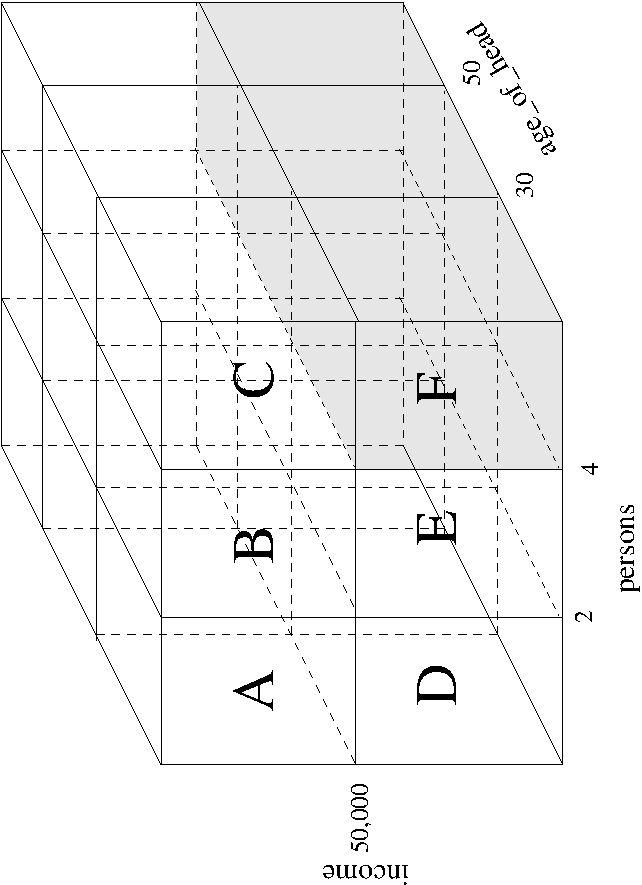
\includegraphics[scale=0.5, angle=-90]{images/htmexample.pdf}
%end{latexonly}
\caption{\label{fig:htm-example}\small Example of dividing household
  characteristics into bins.}
\htmlonly{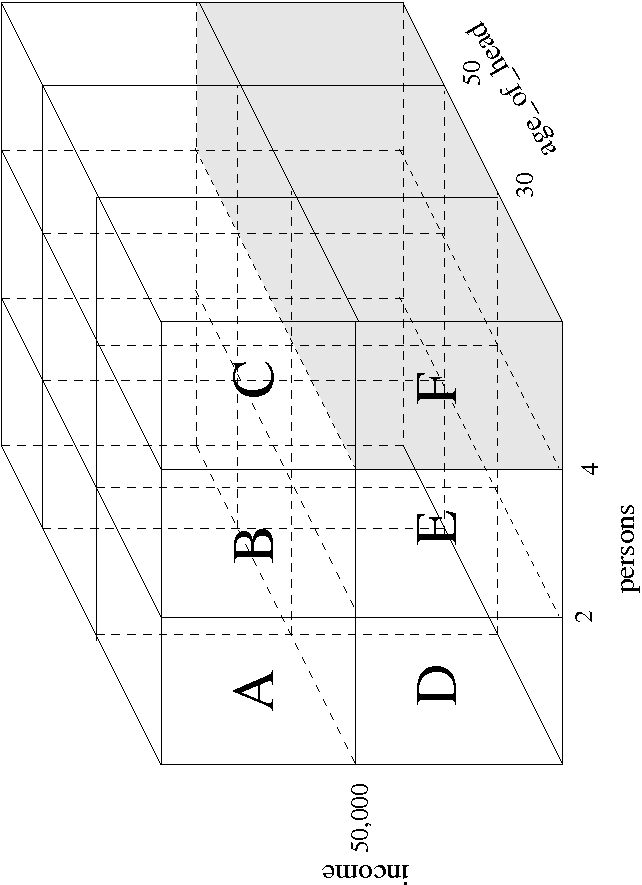
\includegraphics[scale=0.5, angle=-90]{images/htmexample.jpg}}
\end{center}
\end{figure}

The table for the control totals dataset can be
defined as follows:
\begin{verbatim}
year       persons      income     total_number_of_households
2006         0             0                100100
2006         1             0                230000
2006         2             0                 10000
2006         0             1                150000
2006         1             1                250000
2006         3             1                  5000
2007         0             0                110000
  .
  .
  .
\end{verbatim}
The characteristics table defines the groups of each characteristics:
\begin{verbatim}
characteristic      min        max
persons               0          2
persons               2          4
persons               4         -1
income                0      49999
income            50000         -1
age_of_head           0         29
age_of_head          30         49
age_of_head          50         -1
\end{verbatim}
Note that $-1$ stands for $\infty$. The values in the control totals table
denotes the index (starting from 0) of the particular group within the
characteristics table. E.g. the first line in the control totals table refers
to the persons group $[0,2]$ and income group $[0,49999]$.

The model \modelsindex iterates over bins defined by the marginal characteristics. In this
case, it would iterate over the 6 groups marked by A,B,C,D,E,F in
Figure~\ref{fig:htm-example}, it would then determine the number of households
that belong to each group in terms of their characteristics and compare it
with the control total for that group. If for example in bin F (shaded area in
the figure) there are 10 households to be created, the model \modelsindex would randomly
sample (with replacement) 10 bins from the 3 bins within F (formed by groups
on the axis ``age_of_head''), weighted by the number of existing households in
those bins.  These are categories of the 10 new households. Then for each of
the 10 households it would randomly sample the actual value of each
characteristics.  For example, for the very front cube of F, it would sample
income between 0 and $49,999$ (rounded to the nearest 10), number of persons
between 4 and 8\footnote{When a maximum is set to $\infty$, we replace it by a
  reasonable maximum for sampling, which is two times the category range.}
and age of head between 15 and 29.  If the difference between control total
and the number of households in F would call for removing households, the
model \modelsindex would randomly sample households belonging to F regardless to which bin
within F they belong.

\subsubsection{Model Configuration}
\modelsindex
%
{\em Configuration for Production Run}:\\[1mm]
In a production run of UrbanSim, the model \modelsindex runs with the following arguments:
\begin{description}
\item[year] - The current year of the simulation.
\item[household_set] - A \class{HouseholdDataset} object created with data from
  table ``households'' (see Section~\ref{sec:household-tables}
  for the table structure).
\item[control_totals] - A \class{ControlTotalDataset} object inititated with the
  argument \verb|what=|``household'' that reads data from table
  ``annual_household_control_totals'' (see Section~\ref{sec:household-tables}
  for the table structure).
\item[characteristics] - A \class{HouseholdCharacteristicDataset} object created
  with data from table ``household_characteristics_for_ht'' (see
  Section~\ref{sec:household-tables} for the table structure).
\end{description}


%
\subsection{Employment Transition Model}
\modelsindex
%
\label{sec:employment-transition-model}
\index{Employment Transition Model}

The class \class{EmploymentTransitionModel} \modelsindex creates and removes jobs to and
from given job set according to a job distribution over employment sectors.
The total number of jobs is controlled by given annual control totals. It
distinguishes between home based and non-home based jobs.

The algorithm is a simplification of the Household Transition Model. \modelsindex There are
no scaled characteristics and the only marginal characteristics are sector
identifiers.

\subsubsection{The Run Method}
%
{\it Input}:
\begin{description}
\item[year] - an integer indicating the simulated year.
\item[job_set] - an instance of \class{Dataset} \datasetindex that contains some
  specific attributes \attributesindex (see description of the algorithm bellow).
\item[control_totals] - an instance of \class{ControlTotalDataset} initiated for
  the dataset ``employment''. It must have at least attributes \attributesindex ``sector_id'',
  ``total_home_based_employment'', ``total_non_home_based_employment'' and
  ``year'' which specify the annual control totals per sector and employment
  type.  The unique identifier of this dataset \datasetindex should be ``year'' and
  ``sector_id'' (for details see Section ``annual_employment_control_totals''
  in~\ref{sec:employment-tables}).
\item[job_building_types] - an instance of class \class{Dataset} that contains unique 
building types of jobs. It must contain an attribute 'home_based' determining which 
of the building types are home based (see ``job_building_types'' in~\ref{sec:employment-tables}).
 \item[data_objects] - a dictionary containing other datasets \datasetindex and arguments
  needed for computing variables. \variablesindex
\item[resources] - additional \class{Resources} for controlling the
  simulation run. The argument is not used in this version of the model. \modelsindex
\end{description}


{\it Algorithm}:~\\[1mm]
The \verb|job_set| is required to have a primary attribute \primaryattributesindex
``building_type'' with values that correspond to values of the unique identifier of \verb|job_building_types|.
The algorithm invokes a computation of variables \variablesindex
``is_in_employment_sector_$n$_home_based'' and
``is_in_employment_sector_$n$_non_home_based'' implemented in the package
given by the class property \verb|variable_package| \variablesindex (by default
``urbansim''). $n$ in the variable \variablesindex names is the sector id. If you use
the default \package{urbansim} implementation of those variables, \variablesindex they require
a primary attributes \primaryattributesindex ``home_based'' of the dataset \verb|job_building_types|
and a primary attribute ``sector_id'' of \verb|job_set|. Each job is set to be home based if its building 
type is home based, otherwise the job is non-home based.  

The method iterates over sectors given in \verb|control_totals|. For each
sector it determines the number of jobs of that sector that are home based
(non-home based) using the above variables. \variablesindex It then compares those numbers to
the control totals.  If the difference $d_h$ ($d_{nh}$) is positive, new home
based (non-home based) jobs are created, if it is negative, home based
(non-home based) jobs are removed, if it is zero, nothing is done.

Jobs that are created get the corresponding values for the attribute \attributesindex
``sector_id''. For each combination of (sector id, home based) and (sector id, non-home based) 
it is determined, if there are any jobs of this group
previously available. In such a case, the distribution of ``building_type'' among those jobs is
determined and the values for ``building_type'' of the new jobs are sampled
from this distribution. If there are no existing jobs in this group, it is
sampled from the ``building_type'' distribution obtained over all home based
(non-home based) jobs, regardless of the sector id.

To remove home based (non-home based) jobs from a sector, first unplaced home
based (non-home based) jobs of this sector are removed. If the number $n_{h_u}$
($n_{nh_u}$) of those unplaced jobs is larger than $d_h$ ($d_{nh}$), only
$d_h$ ($d_{nh}$) jobs are randomly sampled for deletion. If $n_{h_u}$
($n_{nh_u}$) is smaller than $d_h$ ($d_{nh}$), then $d_h-n_{h_u}$
($d_{nh}-n_{nh_u}$) jobs from the set of placed jobs of that sector are
randomly sampled and deleted. Jobs are considered as unplaced if their
attribute \attributesindex given by the class property \verb|location_id_name| (which is by
default ``grid_id'') is smaller equal zero.

{\it Output}:~\\[1mm]
The method returns the total difference between the sizes of the job
dataset \datasetindex after and before the model \modelsindex run. Thus, a positive value means that in
total there were more jobs added than removed, a negative value means
the opposite.

\subsubsection{Model Configuration}
\modelsindex
%
{\em Configuration for Production Run}:\\[1mm]
In a production run of UrbanSim, the model \modelsindex runs with the following arguments:
\begin{description}
\item[year] - The current year of the simulation.
\item[job_set] - A \class{JobDataset} object created with data from
  table ``jobs'' (see Section~\ref{sec:employment-tables}
  for the table structure).
\item[control_totals] - A \class{ControlTotalDataset} object initiated with the
  argument \verb|what=|``employment'' that reads data from table
  ``annual_employment_control_totals'' (see
  Section~\ref{sec:employment-tables} for the table structure).
\item[job_building_types] - A \class{JobBuildingTypeDataset} created with data from table 
``job_building_types'' (see Section~\ref{sec:employment-tables}
  for the table structure).
\end{description}



%
\subsection{Agent Relocation Model}
\modelsindex
%
\label{sec:agent-relocation-model}
\index{Agent Relocation model}

The class \class{AgentRelocationModel} \modelsindex determines which members of the given
set of agents should be relocated. This is done on basis of given
probabilities. Additionally, the way how to choose the agents can be given by
passing a \class{Choices} object.

%
\subsubsection{Initialization}
%
The class is initialized by passing the following arguments:
\begin{description}
\item[probabilities] - A fully qualified name of the module that implements
  computing relocation probabilities. The module should be a child of the
  \package{opus_core} class \class{Probabilities}.
\item[choices] - A fully qualified name of the module that implements choosing
  agents for relocation according to given probabilities. The module should be
  a child of the \package{opus_core} class \class{Choices}.  Default value is
  ``opus_core.random_choices'' (see Section~\ref{sec:choices}).
\item[location_id_name] - Name of the attribute \attributesindex that specifies locations. It
  must be a primary attribute \primaryattributesindex of the agent set. Default value is
  ``grid_id''.
\item[model_name] \modelsindex - Name of the model. \modelsindex Default value is ``Agent Relocation
  Model''. \modelsindex
\end{description}
The initialization method creates a class attribute \attributesindex \verb|upc_sequence|, using
the passed arguments \verb|probabilities| and \verb|choices|. It is an object
of class \class{upc_sequence} where the utilities component is set to None
(see Section~\ref{sec:upc-sequence}).

%
\subsubsection{The Run Method}
%
{\it Input}:
\begin{description}
\item[agent_set] - A \class{Dataset} \datasetindex object containing agents to be relocated.
\item[resources] - An instance of class \class{Resources} which is a
  collection of additional arguments and objects that will be passed to the
  \verb|upc_sequence| run.
\end{description}

{\it Algorithm}:~\\[1mm]
The method appends \verb|agent_set| into \verb|resources| and invokes the
\method{run()} method of \verb|upc_sequence|, passing \verb|resources| as
argument. The \verb|upc_sequence| runs the probabilities component and the
choices component and it is expected to return an array of zeros for agents
not to be relocated, and ones for agent to be relocated. The distinct values
of indices of the ``to be relocated'' agents joined with indices of all
unplaced agents is the resulting array of agents to be relocated. As unplaced
agents are considered agents that have value smaller equal 0 for the attribute \attributesindex
given in \verb|location_id_name| passed to the constructor.

{\it Output}:~\\[1mm]
The method returns the resulting array of indices of all agents to be
relocated.

%
\subsubsection{Creators}
%
There are two pre-defined creators in \package{urbansim}. Their method
\method{get_model()} \modelsindex returns an instance of
\class{AgentRelocationModel} \modelsindex with the following default settings:
\begin{itemize}
\item \class{HouseholdRelocationModelCreator} \modelsindex - sets the argument
  \verb|probabilities| to ``urbansim.household_relocation_probabilities''
  (see Section~\ref{sec:urbansim-probabilities}) and \verb|model_name| \modelsindex to
  ``Household Relocation Model''. \modelsindex
\item \class{EmploymentRelocationModelCreator} \modelsindex - sets the argument
  \verb|probabilities| to
  ``urbansim.employment_relocation_probabilities'' (see
  Section~\ref{sec:urbansim-probabilities}) and \verb|model_name| \modelsindex to
  ``Employment Relocation Model''.  \modelsindex
\end{itemize}

%
\subsubsection{Model Configuration}
\modelsindex
%
{\em Configuration for Production Run}:
\begin{itemize}
\item To run a {\bf Household Relocation Model} \modelsindex in a production run, the
  \class{HouseholdRelocationModelCreator} \modelsindex is used to create an instance of the
  \class{AgentRelocationModel}. \modelsindex Additionally, it creates an instance of
  \class{RateDataset} initialized with the argument \verb|what=|''households''
  which reads data from table ``annual_relocation_rates_for_households'' (see
  Section~\ref{sec:household-tables} for the table structure). This object is
  put into {\bf resources} which is passed to the \method{run()} method of
  the model. \modelsindex As {\bf agent_set} the production code passes a
  \class{HouseholdDataset} object that was (possibly) used and modified by the
  Household Transition Model. \modelsindex
\item To run a {\bf Employment Relocation Model}, \modelsindex the
  \class{EmploymentRelocationModelCreator} \modelsindex is used to create an instance of the
  \class{AgentRelocationModel}. \modelsindex Additionally, it creates an instance of
  \class{RateDataset} initialized with the argument \verb|what=|''jobs''
  which reads data from table ``annual_relocation_rates_for_jobs'' (see
  Section~\ref{sec:employment-tables} for the table structure). This object is
  put into {\bf resources} which is passed to the \method{run()} method of
  the model. \modelsindex As {\bf agent_set} the production code passes a
  \class{JobDataset} object that was (possibly) used and modified by the
  Employment Transition Model. \modelsindex
\end{itemize}

%
\subsection{Agent Location Choice Model}
\modelsindex
%
\label{sec:agent-lcm}
\index{Agent Location Choice Model}

The class \class{AgentLocationChoiceModel} \modelsindex is a child
of \class{LocationChoiceModel} \modelsindex described in
Section~\ref{sec:location-choice-model}. \modelsindex It extends the
parent class only in one way: It puts the parent method
\method{run()} into a loop which is repeated whenever there is an
overflow in the capacity after the last run. This behavior is
activated only if the ``compute_capacity_flag'' entry of
\verb|run_config| is set to True. In such a case, \verb|run_config|
also should have entries ``number_of_units_string'' giving the
variable \variablesindex name for computing number of available
units in each location, and ``number_of_agents_string'' giving the
variable \variablesindex name for computing the number of agents
located in each location. Those variables \variablesindex are
computed and the difference in their values determines the
overfilled locations. If there are any such locations, an
appropriate number of agents (from the set given by
\verb|agents_index|) are removed from their locations and the parent
\method{run()} method is called again. The maximum number of
iterations is 10.

The model \modelsindex also completes any unqualified variable \variablesindex names given in constructor
arguments, \verb|run_config| and \verb|estimate_config| to fully-qualified
names, by using the dataset name of the given \verb|location_set| and package
``urbansim''.


\subsubsection{Model Configuration}
\modelsindex
%
{\em Configuration for Production Run}:\\[1mm]
The {\bf HouseholdLocationChoiceModelCreator} passes a
\class{BuildingDataset} object that was (possibly) used and modified by the
development models \modelsindex to the constructor of \class{AgentLocationChoiceModel} \modelsindex as
the argument {\bf location_set}. Additionally, it overwrites the default
value of {\bf choices} with ``urbansim.lottery_choices'' (see
Section~\ref{sec:urbansim-choices}).

The following arguments are passed to
  the \method{run()} method:
\begin{description}
\item[specification] - An \class{EquationSpecification} object created with
  data from table ``household_location_choice_model_specification''. \modelsindex
\item[coefficients] \coefficientsindex - A \class{Coefficients} \coefficientsindex object created with data from
  table ``household_location_choice_model_coefficients''. \modelsindex
\item[agent_set] - A \class{HouseholdDataset} object used in Household Relocation
  Model. \modelsindex
\item[agents_index] - Results of Household Relocation Model. \modelsindex Make sure this model is turned on 
when running Household Location Choice Model.
\end{description}

\subsection{Employment Location Choice Model}
\modelsindex
\label{sec:elcm} \index{Employment Location Choice Model}
%
The class \class{EmploymentLocationChoiceModel} is a child of \class{AgentLocationChoiceModel}\index{model group}. 
It is initialized by arguments (see also their default values):
\begin{verbatim}
    location_set, 
    sampler = "opus_core.samplers.weighted_sampler", 
    utilities = "opus_core.linear_utilities", 
    choices = "opus_core.random_choices", 
    probabilities = "opus_core.mnl_probabilities", 
    estimation = "opus_core.bhhh_mnl_estimation", 
    capacity_string = "vacant_job_space",
    estimation_weight_string = "total_number_of_possible_jobs",
    number_of_agents_string = "number_of_jobs",
    number_of_units_string = "total_number_of_possible_jobs",
    sample_proportion_locations = None, 
    sample_size_locations = 30, 
    estimation_size_agents = 1.0, 
    compute_capacity_flag = True, 
    correct_sampling_bias = False,
    filter = None,
    submodel_string = "sector_id", 
    location_id_string = None,
    demand_string = None, 
    run_config = None, 
    estimate_config=None, 
    debuglevel=0, 
    dataset_pool=None):
\end{verbatim}


\subsubsection{Model Configuration}
\modelsindex
%
{\em Configuration for Production Run}:\\[1mm]
The following arguments are passed to the model constructor:
\begin{description}
\item[location_set] - A \class{BuildingDataset} object.
\item[choices] - 'urbansim.lottery_choices'
\end{description}

The \method{run()} method is called with the following arguments:
\begin{description}
\item[specification] - Uses data from
  ``employment_location_choice_model_specification'' .
\item[coefficients] \coefficientsindex - Uses data from ``employment_location_choice_model_coefficients'' 
\item[agent_set] - A \class{JobDataset} object used in Employment Relocation Model. \modelsindex
\item[agents_index] - Results of Employment Relocation Model \modelsindex.
\end{description}
 
\subsection{Scaling Jobs Model}
\modelsindex
%
\label{sec:scaling-jobs-model} \index{Scaling Jobs Model}
%
The class \class{ScalingJobsModel} \modelsindex locates jobs to locations according to the
distribution of jobs sectors in locations. \index{model group}
\subsubsection{Initialization}
The model is initialized by passing the following arguments:
\begin{description}
\item[group_member] - An object of class \class{ModelGroupMember} (see~\ref{sec:model-group}). Default is \verb|None|.
\item[agents_grouping_attribute] - The agents grouping attribute. Default is 'job.building_type'.
\end{description}

\subsubsection{The Run Method}
%
{\it Input}:
\begin{description}
\item[location_set] - an instance of \class{Dataset} containing the set of all
  locations for locating jobs.
\item[agent_set] - an instance of \class{Dataset} containing the set of all
  jobs. It must have an attribute \attributesindex ``sector_id'' and attribute \attributesindex of the same name
  as the unique identifier of the \verb|location_set|.
\item[agents_index] - indices of members of the \verb|agent_set| for which the
  model \modelsindex runs. If it is None, the whole \verb|agent_set| is considered.
\item[data_objects] - a dictionary containing other datasets \datasetindex and arguments
  needed for computing variables. \variablesindex
\item[resources] - additional \class{Resources} for controlling the
  simulation run. The argument is not used in this version of the model. \modelsindex
\end{description}

{\it Algorithm}:~\\[1mm]
The \verb|location_set| is expected to have implemented variable
\variablesindex ``number_of_jobs_of_sector_$n$'' in the package
given by the class property \verb|variable_package| (default is
``urbansim'').  $n$ is an integer giving sector IDs.

The method filters out jobs that are supposed to be located using \verb|agents_index| and 
the 'membership' of jobs given by 'group_member'. (If 'group_member' is \verb|None| the group membership is ignored.)
Then it determines distinct sectors of those jobs and their count in each of
these sectors. It iterates over those sectors. In each iteration it
randomly samples (with replacement) the desired count of locations
weighted by the number of existing jobs of that sector in each
location. If there are no existing jobs in that sector, it samples
with equal weights for all locations.  It then modifies the location
attribute \attributesindex of the job set by storing the sampled
location IDs.

{\it Output}:~\\[1mm]
The method returns an array of the new locations, i.e. of size
\verb|agents_index|. For entries in verb|agents_index| that do not belong to this group member, the values are -1.

\subsubsection{Model Configuration}
\modelsindex
%
{\em Configuration for Production Run}:\\[1mm]
In the production run of UrbanSim, the model is run for group member 'governmental' (if this name is included
in the table \file{job_building_types}).
The \method{run()} method is called with
the following arguments:
\begin{description}
\item[location_set] - A \class{GridcellDataset} object that was (possibly) used
  and modified by the development models. \modelsindex
\item[agent_set] - A \class{JobDataset} object used in Employment Relocation
  Model. \modelsindex
\item[agents_index] - Results of Employment Relocation Model. \modelsindex
\end{description}

\subsection{Events Coordinator}
\label{sec:events-coordinator}
\index{Events Coordinator}
%
The class \class{EventsCoordinator} updates a location set to reflect changes
that are contained in the output of the Development Event Transition Model. \modelsindex
There is no \method{estimate()} method for this model. \modelsindex
%
\subsubsection{The Run Method}
%
{\it Input}:
\begin{description}
\item[model_configuration] \modelsindex - a \class{Configuration} object that determines
  project types and settings for each type (see Model \modelsindex Configuration of
  Section~\ref{sec:development-project-transition-model}).
\item[location_set] - a \class{Dataset} \datasetindex object to be updated.
\item[development_event_set] - a \class{DevelopmentEventDataset} with development
  events to be used to update the locations.
\item[development_type_set] - an object of class \class{DevelopmentTypeDataset}.
\item[current_year] - an integer value determining the year of events by
  which the locations are updated.
\end{description}

{\it Algorithm}:\\[1mm]


{\it Output}:~\\[1mm]
Returns a tuple of indices of locations that were modified, and indices of
development events that were processed.

\subsubsection{Model Configuration}
\modelsindex
%
{\em Configuration for Production Run}:\\[1mm]
For a production run of UrbanSim the method \method{run()} is called using the
following arguments:
\begin{description}
\item[model_configuration] \modelsindex - The model \modelsindex configuration for project types from
  \file{general_configuration.py} as shown on page~\pageref{page:model-configuration}.
\item[location_set] - An instance of class \class{GridcellDataset} created with
  data from table ``gridcells'' (see Section~\ref{sec:gridcell-tables} for the
  table structure) and (possibly) modified by previous models. \modelsindex
\item[development_event_set] - Result of a Development Event Transition Model \modelsindex
  run.
\item[current_year] - The current year of the simulation.
\end{description}


